\section{Design et fonctionnement du système}
\subsection{Diagramme de classe}
\subsubsection{Général}
{
\begin{figure}[H]
    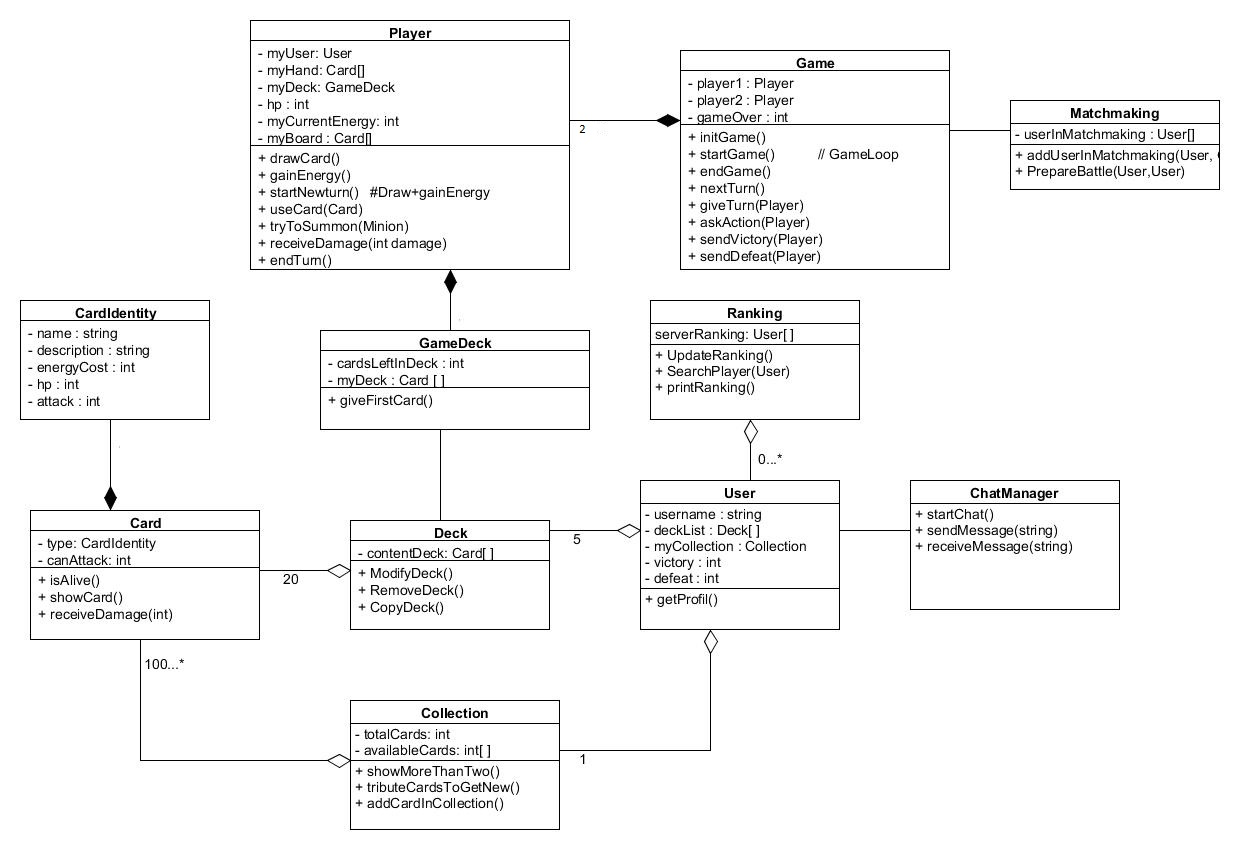
\includegraphics[width=1\textwidth,height=1\textwidth]{Images/classDiagram.jpg}
    \caption{\label{Class Diagram Partie}Diagramme de classe général}
\end{figure}
\noindent\textbf{Analyse}\\
Diagramme de classe illustrant l'interaction entre les principaux objets\index{objet}. Il recense les méthodes\index{méthode} et attributs \index{attribut}
principaux de chaque classe.
}
\subsubsection{Client-Serveur-Database}
{
\begin{figure}[H]
    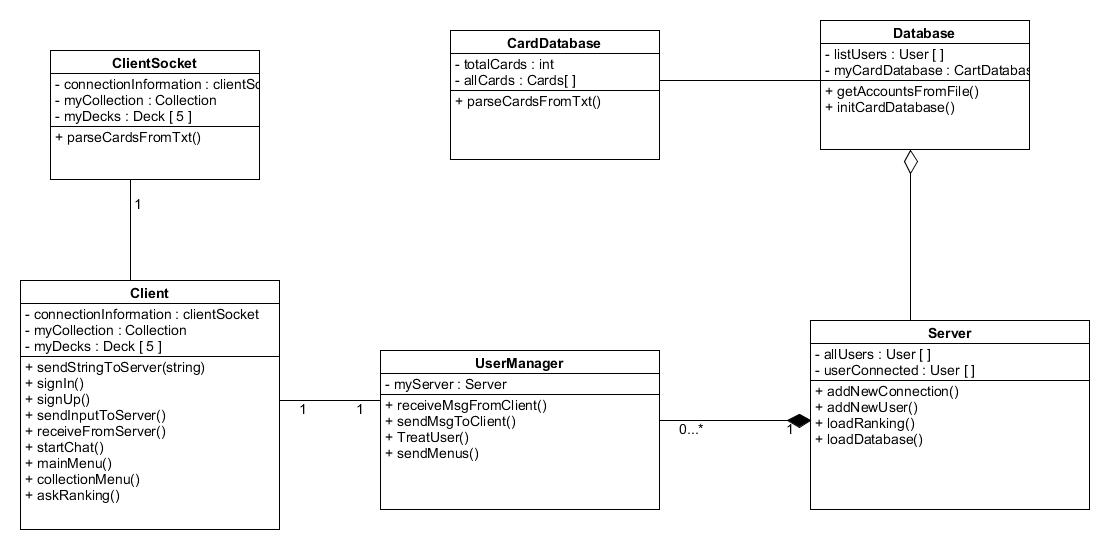
\includegraphics[width=1\textwidth,height=1\textwidth]{Images/classDiagram2.jpg}
    \caption{\label{Class Diagram Partie}Diagramme de classe client-serveur\index{client}\index{serveur}}
\end{figure}
\noindent\textbf{Analyse}\\
Diagramme de classe reprenant l'idée générale des objets\index{objet} instanciés pour les échanges entre le client et le serveur. La database est également représenté comme étant lié au serveur. Celle-ci sera chargé via des fichiers txt.
}
\subsection {Diagramme de séquence}
\subsubsection{Lancement du jeu et invocation}
{
\begin{figure}[H]
    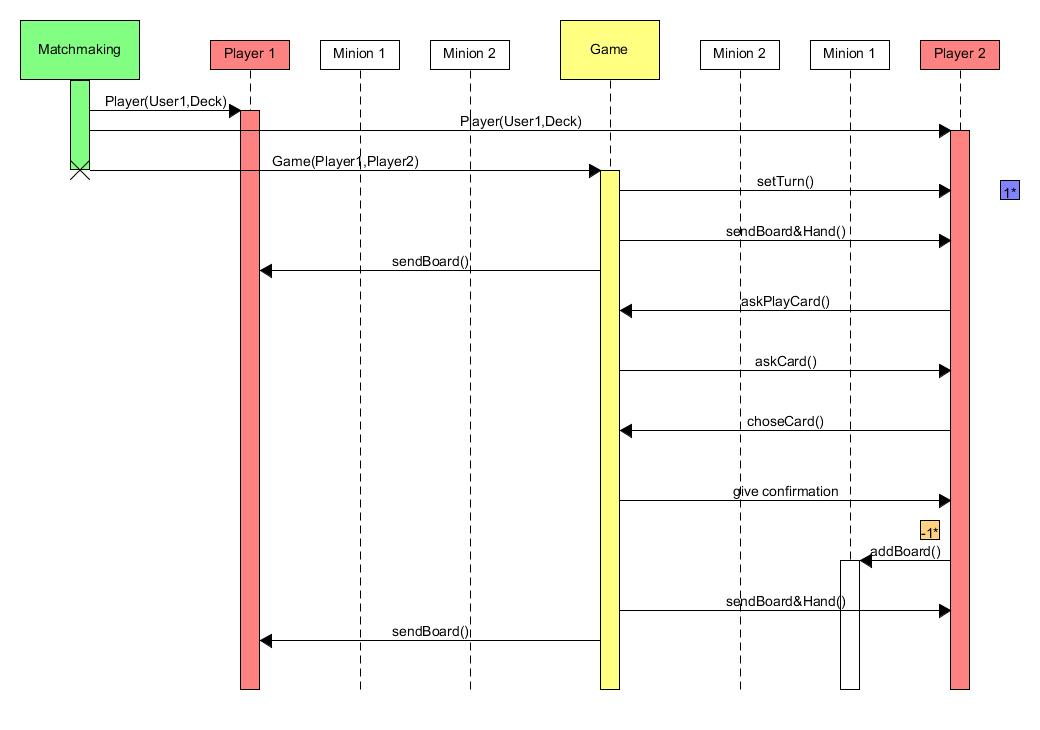
\includegraphics[width=1\textwidth,height=1\textwidth]{Images/CreationAndInvocation.jpg}
    \caption{\label{Sequence Diagram Partie}Diagramme de séquence d'un début de partie et invocation}
\end{figure}
\noindent\textbf{Analyse}\\
Ce diagramme de séquence montre les interactions entre les différents objets\index{objet} au lancement du jeu et lors des invocations de créatures\index{créature}.
}
\subsubsection{Attaque d'une créature envers une autre}
{
\begin{figure}[H]
    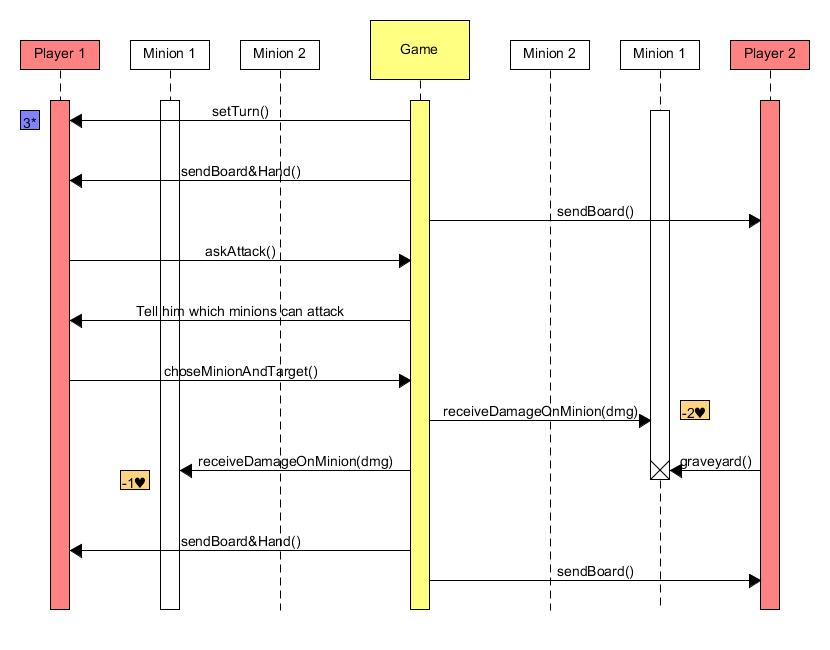
\includegraphics[width=1\textwidth,height=1\textwidth]{Images/AttackOnMinion.jpg}
    \caption{\label{Sequence Diagram Partie} Attaque d'une créature}
\end{figure}
\noindent\textbf{Analyse}\\
Ce diagramme de séquence montre les interactions entre les différents objets \index{objet}lors d'une attaque d'une créature\index{créature} contre une autre.
}

\subsubsection{Attaque d'une créature envers un joueur adverse}
{
\begin{figure}[H]
    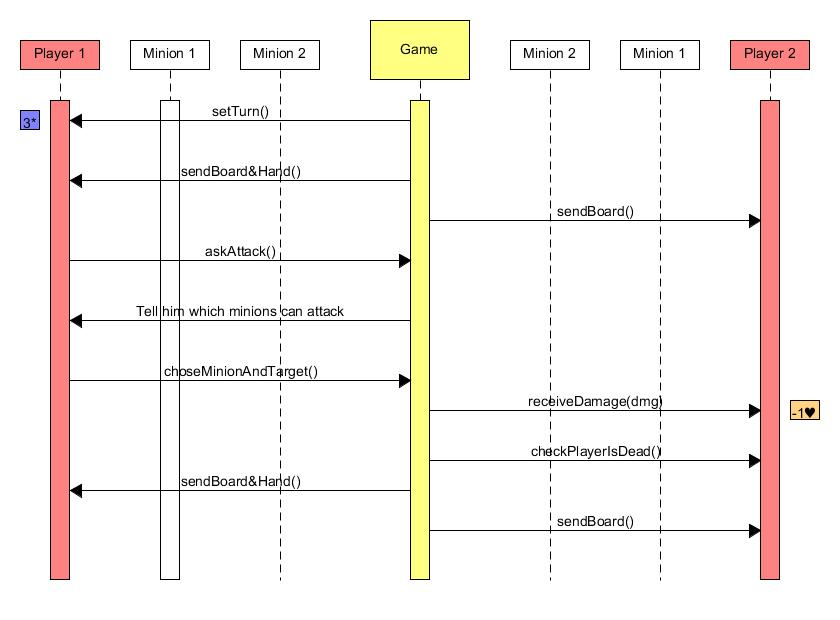
\includegraphics[width=1\textwidth,height=1\textwidth]{Images/AttackOnPlayer.jpg}
    \caption{\label{Sequence Diagram Partie} Attaque d'une créature}
\end{figure}
\noindent\textbf{Analyse}\\
Ce diagramme de séquence montre les interactions entre les différents objets \index{objet} lors d'une attaque d'une créature\index{créature} contre le joueur adverse\index{adversaire}.
}

\subsection{Use Case}
{
\begin{figure}[H]
    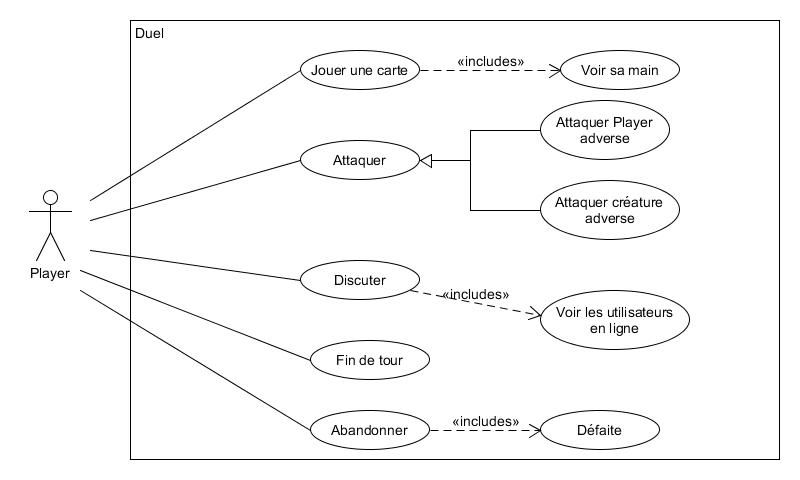
\includegraphics[width=1\textwidth,height=1\textwidth]{Images/UseCaseDuel.jpg}
    \caption{\label{Use Case}Use case représentant les actions\index{action} lors d'un tour}
\end{figure}
\noindent\textbf{Analyse}\\
Ce use case retrace les différentes actions possibles lors d'un tour.

\subsection{Diagramme d'activité}
\begin{figure}[H]
    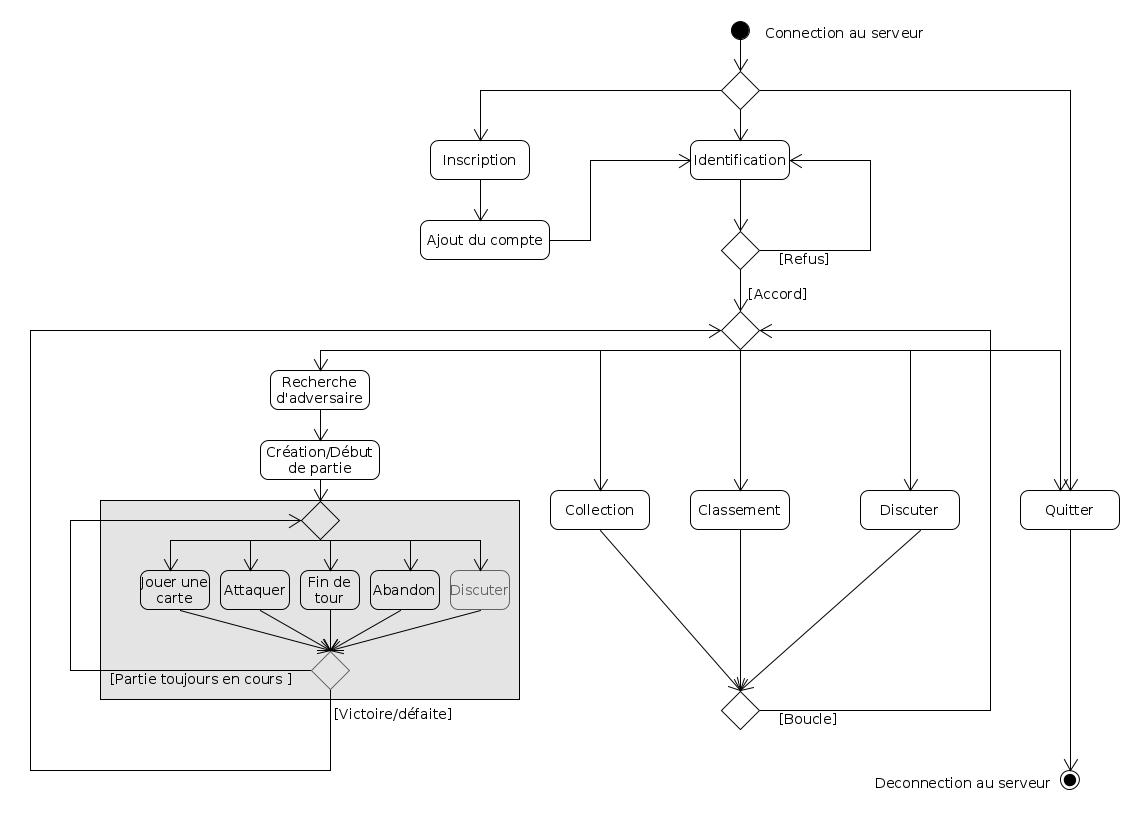
\includegraphics[width=1\textwidth,height=1\textwidth]{Images/activityDiagram.jpg}
    \caption{Diagramme d'activité client-server}
\end{figure}
\noindent\textbf{Analyse}\\
Ce diagramme d'activité représente les différentes opérations en termes d'action\index{action} que l'utilisateur\index{utilisateur} peut réaliser.
